\RequirePackage{expl3}
\ExplSyntaxOn
\cs_generate_variant:Nn \tl_if_eq:nnT { VnT }
\cs_generate_variant:Nn \tl_if_eq:nnF { VnF }
\cs_generate_variant:Nn \tl_if_eq:nnTF { VnTF }
\ExplSyntaxOff

\documentclass[12pt,twoside=false,a4paper,parskip]{scrbook}
% use the following line instead of the class above if you want double-sided printing
% don't remove openright as it looks better in case of double-sided print
% \documentclass[12pt,twoside,a4paper,parskip,openright]{scrbook} 
\usepackage[utf8]{inputenc}
\usepackage[T1]{fontenc}
\usepackage{lmodern}
\usepackage{microtype}
\usepackage{csquotes}
\usepackage[ngerman]{babel}
% \usepackage{floatflt}
\usepackage{subcaption} % modern alternative to subfigure
\usepackage[pdftex]{graphicx}
\usepackage[hidelinks]{hyperref}
\usepackage{xcolor}
\usepackage{amssymb}
\usepackage{textcomp}
\usepackage{nicefrac}
% \usepackage{scrhack}
\usepackage{pdfpages}
\usepackage{float}
\usepackage{pdflscape}
\usepackage[verbose]{placeins}
\usepackage[markcase=ignoreuppercase,headsepline,plainfootsepline]{scrlayer-scrpage}
\usepackage{listings}
\usepackage{caption}
% \usepackage{epstopdf}
\usepackage{longtable}
\usepackage{setspace}
\usepackage{booktabs}
\usepackage[style=numeric,backend=biber,sorting=none]{biblatex}
\bibliography{literatur}
\usepackage[htt]{hyphenat} % texttt do line breaks
\usepackage{tabularx}
\usepackage{multirow}
\usepackage{enumitem}


%%%%%%%%%%%%%%%%%%%
%% definitions
%%%%%%%%%%%%%%%%%%%
\def\BaAuthor{Martin Rapps}
\def\BaAuthorStudyProgram{Geoviusalisierung} 
\def\BaType{Portfolioabgabe Wissenschaftliche Arbeiten} 
\def\BaTitle{Zusammenfassung des Papers: Machine Learning Klassifikation von KI-generierten und menschengemachten Gebäuden in OpenStreetMap}
\def\BaSupervisorOne{Prof. Dr. Wilkening}
\def\BaDeadline{20.04.2026}

\def\iswithfullname{1} % uncomment this to create non-anonymous version
\ifdefined\iswithfullname
  \def\ShowBaAuthor{\BaAuthor}
\else
  \def\ShowBaAuthor{N.~N.}
\fi

\hypersetup{
pdfauthor={\ShowBaAuthor},
pdftitle={\BaTitle},
pdfsubject={Subject},
pdfkeywords={Keywords}
}

%%%%%%%%%%%%%%%%%%%
%% configs to include
%%%%%%%%%%%%%%%%%%%
\colorlet{punct}{red!60!black}
\definecolor{background}{HTML}{EEEEEE}
\definecolor{delim}{RGB}{20,105,176}
\colorlet{numb}{magenta!60!black}

\definecolor{gray}{rgb}{0.4,0.4,0.4}
\definecolor{darkblue}{rgb}{0.0,0.0,0.6}
\definecolor{cyan}{rgb}{0.0,0.6,0.6}

\definecolor{pblue}{rgb}{0.13,0.13,1}
\definecolor{pgreen}{rgb}{0,0.5,0}
\definecolor{pred}{rgb}{0.9,0,0}
\definecolor{pgrey}{rgb}{0.46,0.45,0.48}

\lstset{
  basicstyle=\ttfamily,
  columns=fullflexible,
  showstringspaces=false,
  commentstyle=\color{gray}\upshape
  linewidth=\textwidth
}

\lstdefinelanguage{json}{
    basicstyle=\normalfont\ttfamily,
    numbers=left,
    numberstyle=\scriptsize,
    stepnumber=1,
    numbersep=8pt,
    showstringspaces=false,
    breaklines=true,
    backgroundcolor=\color{background},
    literate=
     *{0}{{{\color{numb}0}}}{1}
      {1}{{{\color{numb}1}}}{1}
      {2}{{{\color{numb}2}}}{1}
      {3}{{{\color{numb}3}}}{1}
      {4}{{{\color{numb}4}}}{1}
      {5}{{{\color{numb}5}}}{1}
      {6}{{{\color{numb}6}}}{1}
      {7}{{{\color{numb}7}}}{1}
      {8}{{{\color{numb}8}}}{1}
      {9}{{{\color{numb}9}}}{1}
      {:}{{{\color{punct}{:}}}}{1}
      {,}{{{\color{punct}{,}}}}{1}
      {\{}{{{\color{delim}{\{}}}}{1}
      {\}}{{{\color{delim}{\}}}}}{1}
      {[}{{{\color{delim}{[}}}}{1}
      {]}{{{\color{delim}{]}}}}{1},
}

\lstset{language=xml,
  morestring=[b]",
  morestring=[s]{>}{<},
  morecomment=[s]{<?}{?>},
  stringstyle=\color{black},
  numbers=left,
  numberstyle=\scriptsize,
  stepnumber=1,
  numbersep=8pt,
  identifierstyle=\color{darkblue},
  keywordstyle=\color{cyan},
  backgroundcolor=\color{background},
  morekeywords={xmlns,version,type}% list your attributes here
}

\lstset{language=Java,
  showspaces=false,
  showtabs=false,
  tabsize=4,
  breaklines=true,
  keepspaces=true,
  numbers=left,
  numberstyle=\scriptsize,
  stepnumber=1,
  numbersep=8pt,
  showstringspaces=false,
  breakatwhitespace=true,
  commentstyle=\color{pgreen},
  keywordstyle=\color{pblue},
  stringstyle=\color{pred},
  basicstyle=\ttfamily,
  backgroundcolor=\color{background},
%  moredelim=[il][\textcolor{pgrey}]{$$},
%  moredelim=[is][\textcolor{pgrey}]{\%\%}{\%\%}
}

\newcommand*{\forcetwosidetitle}[1][1]{%
 \begingroup
   \cleardoubleoddpage
   \KOMAoptions{titlepage=true}% useful e.g. for scrartcl
   \csname @twosidetrue\endcsname
   \maketitle[{#1}]
 \endgroup
}


\begin{document}


%%%%%%%%%%%%%%%%%%%
%% Titelseite
%%%%%%%%%%%%%%%%%%%


\frontmatter
\titlehead{%  {\centering Seitenkopf}
  {Technische Hochschule Würzburg-Schweinfurt\\
    Fakultät Kunststofftechnik und Vermessung}}
\subject{\BaType}
\title{\BaTitle\\[15mm]}
\subtitle{\normalsize{vorgelegt an der Technischen Hochschule W\"{u}rzburg-Schweinfurt in der Fakult\"{a}t Kunststofftechnik und Vermessung zum Abschluss des Moduls Wissenschaftliches Arbeiten im Studiengang \BaAuthorStudyProgram}}
\author{\ShowBaAuthor}
\date{\normalsize{Eingereicht am: \BaDeadline}}
\publishers{
  % Uncomment the following line if you want the QR code to be placed on the title page
  %\centering
\includegraphics[width=4cm]{barcode_default}\\[1cm]
  \normalsize{Erstprüfer: \BaSupervisorOne}\\
}

\forcetwosidetitle


%%%%%%%%%%%%%%%%%%%
%% abstract
%%%%%%%%%%%%%%%%%%%

\addchap{Zusammenfassung}

Diese Portfolioabgabe fasst die Ergebnisse der Studie \cite{memduhoglu2026ml} zusammen, welche die geometrischen Differenzen zwischen KI-generierten und manuell erstellten Gebäudegrundrissen in OpenStreetMap (OSM) untersucht. Auf Basis einer morphometrischen Analyse von über 9 Millionen Gebäuden aus 15 geografisch diversen Städten wird die Leistungsfähigkeit verschiedener Machine-Learning-Modelle evaluiert. Die Ergebnisse zeigen, dass algorithmische Signaturen wie Formregularität und Vertex-Dichte eine Differenzierung mit einer Balanced Accuracy von bis zu 74\,\% ermöglichen. Dabei wird deutlich, dass lokale Digitalisierungspraktiken und die Koexistenz von Mensch und Maschine das Endergebnis maßgeblich beeinflussen.



%%%%%%%%%%%%%%%%%%%
%% Inhaltsverzeichnis
%%%%%%%%%%%%%%%%%%%
\tableofcontents



%%%%%%%%%%%%%%%%%%%
%% Main part of the thesis
%%%%%%%%%%%%%%%%%%%
\mainmatter


\chapter{Relevanz \& wissenschaftlicher Kontext} \label{sec:relevanz}

Die Wahl dieses Papers basiert auf meinem ausgeprägten Interesse an den Potenzialen und Schnittstellen von maschinellen Klassifizierungsmodellen im direkten Zusammenhang mit menschlichem Nutzerverhalten. Die Integration von Künstlicher Intelligenz in Volunteered Geographic Information (VGI)-Plattformen, insbesondere OpenStreetMap (OSM), hat zu einer fundamentalen Transformation der kollaborativen Kartografie geführt. Historisch basierte OSM primär auf der manuellen Digitalisierung durch freiwillige Mapper. Die Einführung von KI-gestützten Extraktionswerkzeugen durch Tech-Akteure beschleunigt die Vervollständigung von Basiskarten massiv. Diese Entwicklung wirft jedoch tiefgreifende wissenschaftliche Fragen hinsichtlich der Datenqualität und der geometrischen Konsistenz auf.

Die Unterscheidung dieser Daten ist operationell essenziell zur Entwicklung von Qualitätskontrollsystemen \cite[S.~2]{memduhoglu2026ml}. Sie ermöglicht es dabei, Ressourcen effizient auf fehlerhafte Gebäude zu lenken. Eine zentrale Erkenntnis der Arbeit ist es, dass eine systematische Zusammenarbeit von Mensch und Maschine oft die belastbarsten Resultate liefert, was rein algorithmisch nicht vollumfänglich prüfbar ist. Historische Datengrundlagen und das spezifische Nutzerverhalten vor Ort haben einen maßgeblichen Einfluss auf das Endergebnis \cite[S.~2]{memduhoglu2026ml}.


\chapter{Synthese \& Struktur} \label{sec:synthese}

Die Studie operiert auf einer massiven Datengrundlage: Sie analysiert insgesamt 9.116.074 Gebäudegrundrisse aus 15 geografisch stark diversen Städten, welche alle sechs Kontinente abdecken. Der dokumentierte Anteil an KI-generierten Gebäuden im Gesamtdatensatz liegt bei 2,69\,\%. Es zeigt sich dabei eine völlig heterogene geografische Varianz in der Akzeptanz und Adoptionsrate solcher KI-Daten.

Das Paper, das klassisch in Einleitung, Hintergrund, Methodik, Ergebnisse, Diskussion und Fazit gegliedert ist \cite[S.~5]{memduhoglu2026ml}, bietet eine systematische Aufarbeitung. Wie in der umfassenden Gesamtdatenmenge ersichtlich wird, gibt es gravierende regionale Unterschiede: So reicht die festgestellte KI-Prävalenz von marginalen 0,15\,\% in Städten wie Tokio bis hin zu dominanten 15,70\,\% in Kairo \cite[S.~5]{memduhoglu2026ml}. Solche weitreichenden Diskrepanzen verdeutlichen, dass neben der reinen Technologieverfügbarkeit vor allem lokale Digitalisierungsgewohnheiten und kulturelle Ansätze kollaborativer Datenerhebung den Einsatz von KI in der Kartografie stark definieren.


\chapter{Hypothese \& ML-Methodik} \label{sec:hypothese}

Die zentrale Hypothese der Forschungsarbeit lautet, dass KI-generierte Gebäude im Vergleich zu unmittelbar menschlich digitalisierten Strukturen distinktive geometrische Muster aufweisen. Diese geometrischen Signaturen ließen sich auf Prinzipien wie algorithmische Regularisierung und konsistente Digitalisierungsgranularität zurückführen und sollten somit durch Machine Learning zuverlässig klassifizierbar sein.

Zur tiefgreifenden Operationalisierung wurden 32 unterschiedliche morphometrische Merkmale systematisch evaluiert (eine exakte Auflistung und Systematisierung dieser Merkmale, e.g. Formregularität und strukturelle Komplexität, ist in Anhang \ref{appendix:merkmale} als detaillierte Tabelle hinterlegt). Die Analyse offenbarte insbesondere die formelle Orthogonalität sowie die Vertex-Dichte als stärkste diskriminative Parameter \cite[S.~10]{memduhoglu2026ml}. Bei der Vorhersage-Modellierung erwies sich LightGBM als das leistungsstärkste Modell und erreichte eine nennenswerte Balanced Accuracy von 74,46\,\% sowie eine \textit{Area Under the Curve} (AUC) von 0,819. Wohingegen der Einsatz von XGBoost an der Klassenstruktur völlig scheiterte, vollständig zur Majoritätsklasse degenerierte und einen kaum noch messbaren Recall von nur 0,68\,\% erreichte \cite[S.~11]{memduhoglu2026ml}.



\chapter{Visualisierungs-Audit} \label{sec:visualisierung}

Das Paper nutzt insgesamt 11 aussagekräftige Abbildungen und 4 Tabellen, um seine Ergebnisse auf verschiedenen Abstraktionsebenen zu untermauern. Neben Gegenüberstellungen typischer morphometrischer Feature-Scores (wie in Figure 4 abgebildet), erweisen sich besonders raumübergreifende Visualisierungen als sinnvoll.

\begin{figure}[htbp]
  \centering
  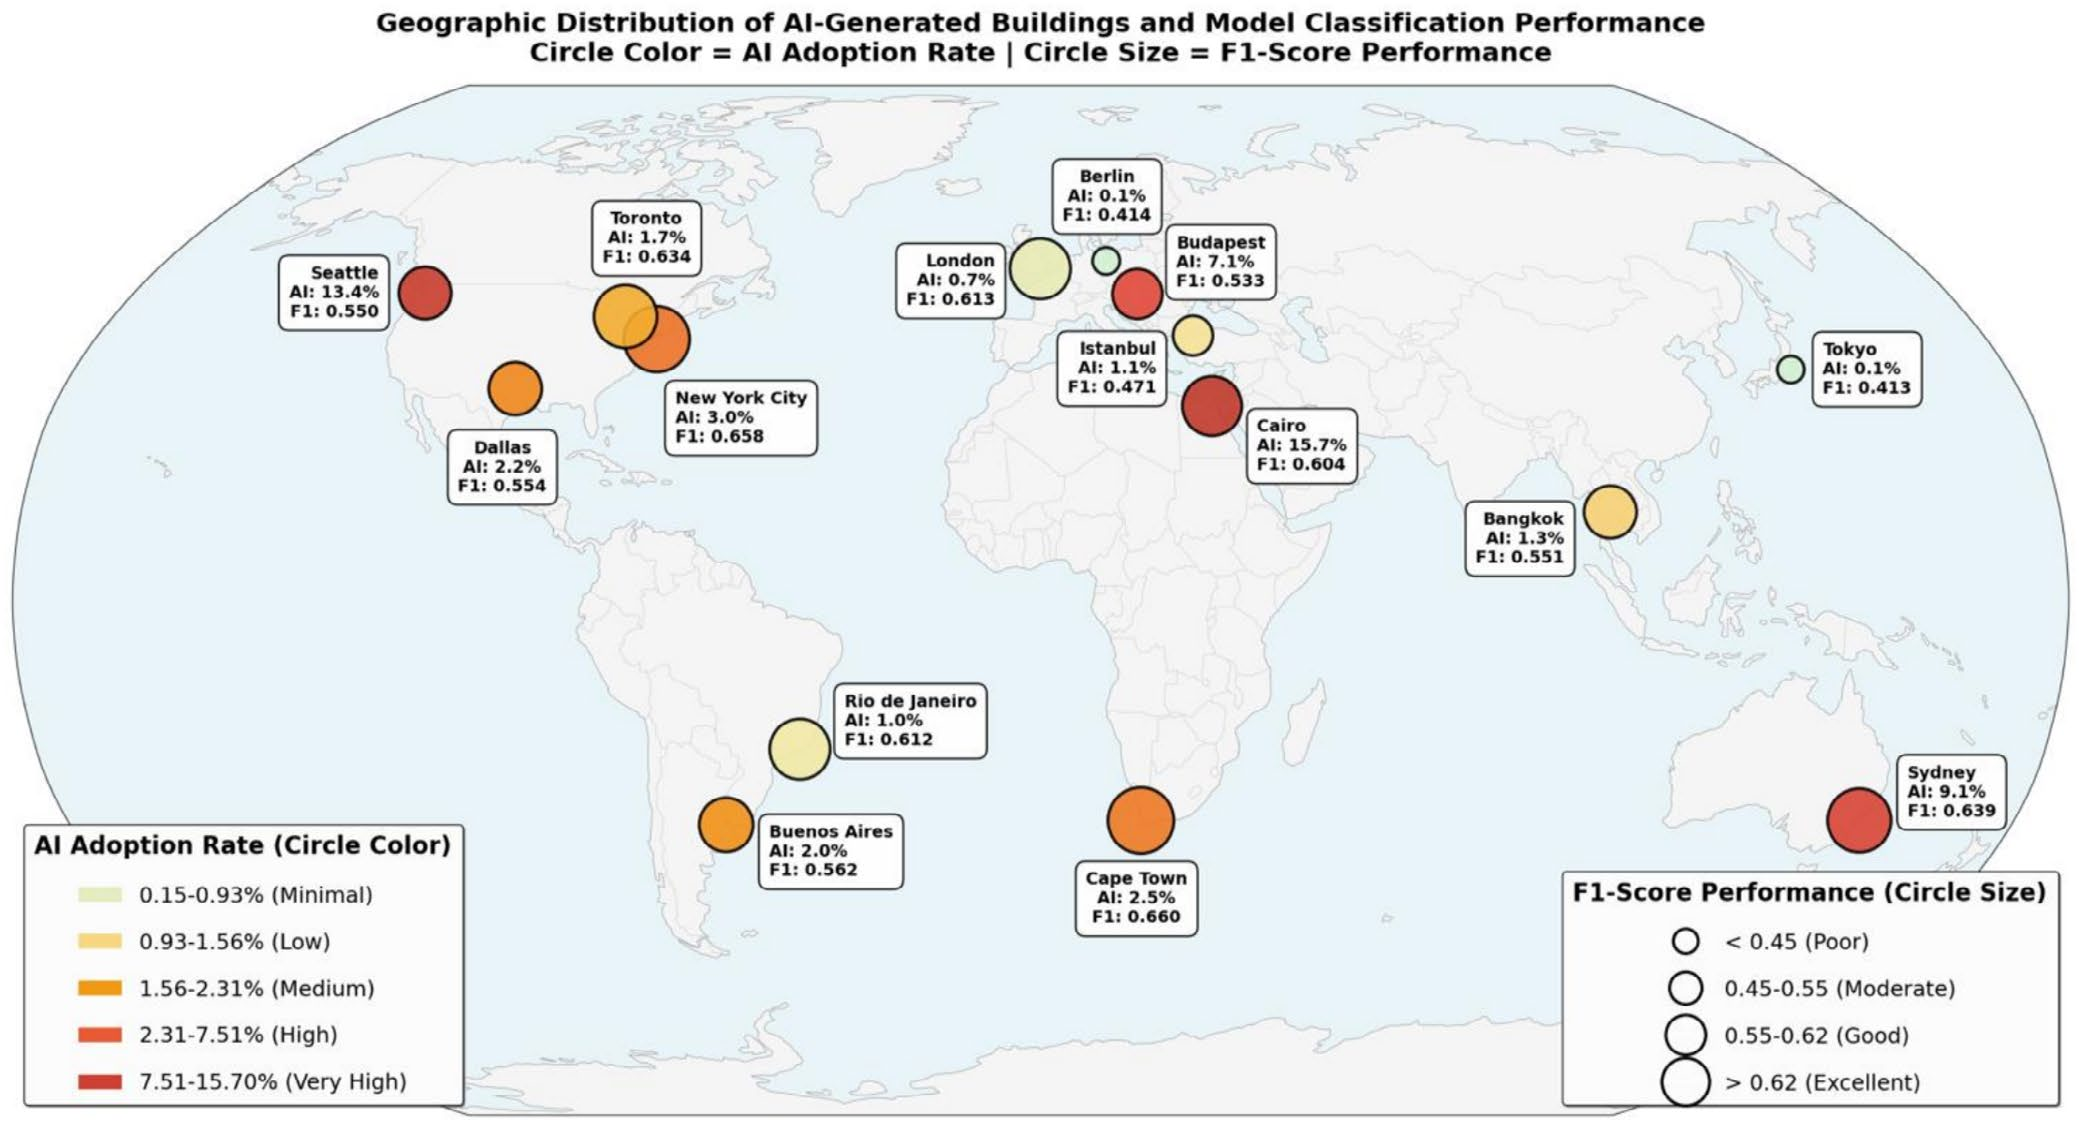
\includegraphics[width=0.75\textwidth]{figure11.jpg}
  \caption{Globale Divergenz von KI-Adoption und Leistungs-F1-Score in ausgewählten Städten (Quelle: \cite[S.~18]{memduhoglu2026ml}).}
  \label{fig:adoptionsrate}
\end{figure}

Wie in der eingebundenen Abbildung \ref{fig:adoptionsrate} bemerkenswert demonstriert wird, korreliert die rechnerische Klassifikationsleistung (F1-Score, hier durch die Kreisgröße repräsentiert) nicht kausal mit der gemessenen KI-Adoptionsrate der entsprechenden Region (angezeigt durch die Farbskala). Anhand dieser Grafik wird etwas Signifikantes ersichtlich: Es verdeutlicht bildhaft, dass die lokalen Praktiken – also wie Menschen mit der KI umgehen, die Daten nachbearbeiten und welche historischen Vermessungstraditionen vorliegen – das methodische Auffinden von KI-Daten weitaus kräftiger modifizieren, als die schiere Masse der vorhandenen maschinellen Daten \cite[S.~13, 16, 18]{memduhoglu2026ml}. Dies stützt die fundamentale Annahme, dass die Koexistenz von Mensch und Maschine das Endprodukt determiniert.


\chapter{Limitationen \& Methodische Konvergenz} \label{sec:limitationen}

Die signifikanteste Limitation der Klassifikation manifestiert sich unweigerlich in der hohen Falsch-Positiv-Rate. Menschliche Mapper und KI-Algorithmen streben beide per Definition nach gewissen Graden an geometriebasierter Regularität. Wenn erfahrene Freiwillige bewusst rechtwinklige Gebäude einzeichnen, um kartografische Klarheit zu erzielen, kreieren sie unbeabsichtigt exakt dieselbe morphometrische Signatur wie KI-Methoden. Eine strikte Formperfektion ist damit längst kein exklusiver Marker für Maschinen mehr.

Dies resultiert in der zutiefst kritischen Problematik der sogenannten \enquote{Label Uncertainty}. Hybride Digitalisierungs-Workflows -- beispielsweise, wenn ein maschineller Ansatz die Basis liefert und der Nutzer diese nachträglich anpasst -- erzeugen zusammen mit den Lücken in der OSM-Versionshistorie unklare Zugehörigkeiten. Da oftmals lediglich der finale und neueste Bearbeiter im System protokolliert wird, führt dies zur Erkenntnis, dass eine verifizierte Provenienz (also der echte Ursprung der Daten) durch rein morphometrische Datenanalyse nie lückenlos und zweifelsfrei nachzuweisen sein wird \cite[S.~20]{memduhoglu2026ml}.


\chapter{Metadaten \& Provenienz} \label{sec:metadaten}

Die untersuchte Forschungsarbeit trägt den Titel \enquote{Machine Learning Classification of AI-Generated and Human-Mapped Buildings in OpenStreetMap Using Morphometric Analysis} \cite[S.~1]{memduhoglu2026ml} und wurde von dem Wissenschaftler Abdulkadir Memduho\u{g}lu verfasst. Memduho\u{g}lu ist am \textit{Department of Geomatic Engineering, Faculty of Engineering} der renommierten Harran University in \c{S}anl{\i}urfa, Türkei, angegliedert.

Die zugrundeliegende Publikation erschien im Jahr 2026 als Bestandteil des hochkarätigen Fachjournals \textit{Transactions in GIS} (Band 30, Artikel-Nr. e70227, DOI: \href{https://doi.org/10.1111/tgis.70227}{10.1111/tgis.70227}). Dieses ist ein Open-Access-Journal, herausgegeben vom bekannten Wissenschaftsverlag John Wiley \& Sons Ltd. Dieses Fachmagazin hat sich auf tiefgehende raumanalytische Studien spezialisiert.

Die methodische Implementierung erfolgte mittels Python 3.10; der entsprechende Quellcode ist zur Förderung der Reproduzierbarkeit öffentlich verfügbar \cite[S.~5]{memduhoglu2026ml}.


\chapter{Reviewer-Gutachten} \label{sec:reviewer}

Aus der disziplinspezifischen Perspektive der Geoinformatik bedarf die methodische Bewertung des vorliegenden Ansatzes einer äußerst differenzierten und scharfen Betrachtung. Das zur Trainingsphase angewandte künstlich balancierte Sampling-Verfahren ist zwar technisch eine völlig klassische und legitime Praxis in der Data Science, um ML-Modellen überhaupt die extrem unterrepräsentierte Minoritätsklasse \enquote{beizubringen}. Wissenschaftlich hochproblematisch ist jedoch die Tatsache, dass es den Anschein erweckt, die operative Anwendbarkeit sei leicht reproduzierbar.

Wird eben jenes Modell auf einen tatsächlichen Real-World-Szenariendatensatz losgelassen – in welchem die Prävalenz von KI-Gebäuden in OSM bei extrem geringen 2,69\,\% liegt – so gerät das System unvermeidlich an seine strukturellen Grenzen. Die Aussagekraft der positiven Vorhersagen (Positive Predictive Value) reduziert sich extrem. Ein vollautomatisierter, unbeaufsichtigter Qualitätskontroll-Filter für Mapping-Tools ist auf dieser Stufe der Genauigkeit folglich noch in weiter Ferne und empirisch entwertet.

Aus den Limitationen und Herausforderungen leiten sich unweigerlich wertvolle und strukturierte methodische Kritikpunkte für sämtliche zukünftigen Studien in diesem Fachbereich ab. Erstens sollte eine realitätsnahe analytische Evaluation der Vorhersagemodelle künftig prinzipiell unter der Berücksichtigung der tatsächlichen KI-Prävalenz anstelle eines künstlichen Test-Sets evaluiert werden. Zweitens birgt die bloße Zusammenfassung unterschiedlicher, massiv heterogener KI-Tools die Gefahr in sich, hochspezifische algorithmische Signaturen unwiederbringlich zu verschleiern und den Algorithmus so zu irritieren. Viertens und letztens bleibt im Anschluss an diese Befunde eine komplett unabhängige und unbeeinflusste Ground-Truth-Studie elementar wichtig. Nur so kann am Ende einwandfrei nachgewiesen werden, ob die aus den geometrischen Morphometriewerten gezogenen Schlüsse nicht potenziell systematisch verfälscht sind \cite[S.~20--21]{memduhoglu2026ml}.


\backmatter
%%%%%%%%%%%%%%%%%%%
%% create figure list
%%%%%%%%%%%%%%%%%%%

\listoffigures
\addcontentsline{toc}{chapter}{Verzeichnisse}

%%%%%%%%%%%%%%%%%%%
%% create appendix
%%%%%%%%%%%%%%%%%%%


\appendix
\addchap{Anhänge}

\addsec{Anhang A: Verwendete Matrix der Merkmale} \label{appendix:merkmale}

Die folgende Tabelle dokumentiert als Referenz sämtliche 32 morphometrischen Merkmale (originale \enquote{Table 2}), die für das algorithmische Modell der Forschungsarbeit genutzt wurden. Die Systematisierung in unterschiedliche geometrische Parameterkategorien untermauert die Vielschichtigkeit der maschinellen Trennbarkeit.

\begin{table}[htbp]
  \centering
  \small
  \begin{tabularx}{\textwidth}{l c X}
    \toprule
    \textbf{Kategorie}                      & \textbf{Anzahl} & \textbf{Merkmale (Features)}                                                                                                                                        \\
    \midrule
    3.3.1—Größe und Dimensionen             & 7               & Area, Perimeter, Log(Area), Sqrt(Area), Perimeter-Area Ratio, Perimeter per Sqrt(Area), Area-Perimeter Ratio²                                                       \\
    \addlinespace
    3.3.2—Form-Regularität                  & 10              & Rectangularity, Rectangularity (Manual), Squareness, Orthogonality, Circular Compactness, Polsby–Popper Compactness, Compactness Ratio, Shape Index, Convexity, ERI \\
    \addlinespace
    3.3.3—Komplexität \& Angularität        & 9               & Fractal Dimension (Momepy), Fractal Dimension (Standard), Vertex Count, Vertex Density, Corners, Vertex Efficiency, Elongation, Elongation², Orientation            \\
    \addlinespace
    3.3.4—Abgeleitete Features \& Anomalien & 6               & Rectangularity–Orthogonality Interaction, Compactness–Fractal Interaction, Orthogonality Z-score, Rectangularity Z-score, Vertex Density Z-score, Anomaly Score     \\
    \midrule
    \textbf{Gesamt}                         & \textbf{32}     &                                                                                                                                                                     \\
    \bottomrule
  \end{tabularx}
  \caption{Matrix der 32 morphometrischen Merkmale (adaptiert nach \cite[S.~7]{memduhoglu2026ml}).}
\end{table}

%%%%%%%%%%%%%%%%%%%
%% create tables list
%%%%%%%%%%%%%%%%%%%
\listoftables

%%%%%%%%%%%%%%%%%%%
%% create listings list
%%%%%%%%%%%%%%%%%%%
%\lstlistoflistings
%\addcontentsline{toc}{chapter}{Listings}

\cleardoublepage
\phantomsection
\addcontentsline{toc}{chapter}{Literatur}
\printbibliography

%%%%%%%%%%%%%%%%%%%
%% declaration on oath
%%%%%%%%%%%%%%%%%%%

\addchap{Eidesstattliche Erklärung}

Hiermit versichere ich, dass ich die vorgelegte Arbeit selbstständig verfasst und noch nicht anderweitig zu Prüfungszwecken vorgelegt habe. Alle benutzten Quellen und Hilfsmittel sind angegeben, wörtliche und sinngemäße Zitate wurden als solche gekennzeichnet.

\vspace{20pt}
\begin{flushright}
  $\overline{~~~~~~~~~~~~~~~~~\mbox{\ShowBaAuthor, am \today}~~~~~~~~~~~~~~~~~}$
\end{flushright}

\addchap{Zustimmung zur Plagiatsüberprüfung}

Hiermit willige ich ein, dass zum Zwecke der Überprüfung auf Plagiate meine vorgelegte Arbeit in digitaler Form an PlagScan (www.plagscan.com) übermittelt und diese vorübergehend (max. 5~Jahre) in der von PlagScan geführten Datenbank gespeichert wird sowie persönliche Daten, die Teil dieser Arbeit sind, dort hinterlegt werden.

\begin{small}
  Die Einwilligung ist freiwillig. Ohne diese Einwilligung kann unter Entfernung aller persönlichen Angaben und Wahrung der urheberrechtlichen Vorgaben die Plagiatsüberprüfung nicht verhindert werden. Die Einwilligung zur Speicherung und Verwendung der persönlichen Daten kann jederzeit durch Erklärung gegenüber der Fakultät widerrufen werden.
\end{small}

\vspace{20pt}
\begin{flushright}
  $\overline{~~~~~~~~~~~~~~~~~\mbox{\ShowBaAuthor, am \today}~~~~~~~~~~~~~~~~~}$
\end{flushright}

\end{document}
